%% This is file `modeloDAINF.tex'
%% Author:  Fabiano Rosas, Gabriel Casella, Lucas Castro, and Aleffer Rocha
%% E-mail:  fabianorosas@gmail.com, gbc921@gmail.com, l.castropg@gmail.com ad aleffer@alunos.utfpr.edu.br
%% File version: 1.1
%% License: Released under the LaTeX Project Public License v1.3c or later
%% See:     http://www.latex-project.org/lppl.txt
%% Last update: June 12, 2019
%% ----------------------------------------------------------------


\documentclass{utfpr-pg}
\usepackage{graphicx}
\usepackage{cmap}
\usepackage{blindtext}
\usepackage[T1]{fontenc}

\usepackage{amssymb}
\usepackage{amsthm}
\usepackage{amsmath}
\usepackage[dvipsnames]{xcolor}

\usepackage{fancyvrb}
\usepackage{nameref}
\usepackage{caption}
\usepackage{listings}
\usepackage{xcolor}

%%daquele jeito
\usepackage{amsmath}
\usepackage{mathtools}
\usepackage[brazilian]{babel}
\usepackage{graphicx}
\usepackage{blindtext}
\usepackage{float}
\usepackage{listings}
\usepackage{hyperref}

\captionsetup{justification=raggedright,singlelinecheck=false,format=hang,skip=-1pt,font={footnotesize,bf},labelfont=bf}


\newlistof{lstlistoflistings}{lol}{\lstlistlistingname}


\let\oldlstlistoflistings\lstlistoflistings
\renewcommand{\lstlistoflistings}{%
  \begingroup%
  \let\oldnumberline\numberline%
  \renewcommand{\numberline}{\lstlistingname~\oldnumberline}%
  \oldlstlistoflistings*%
  \endgroup}


\renewcommand{\lstlistingname}{Código}
\renewcommand{\lstlistlistingname}{Lista de Códigos}

\lstset{
  numbers=left,
  stepnumber=2,
  firstnumber=1,
  numberfirstline=true
  captionpos=b,                    % sets the caption-position to bottom
}


\DeclareFloatingEnvironment[
fileext=lod,
listname=Lista de Definições,
name=Definição,
placement=tbhp,
]{definicao}



\departamento{Departamento Acadêmico de Informática}

%Caso TCC altere para o nome do seu curso de graduação!!!!
\curso{Bacharelado em Ciência da Computação}

\autor{Jefferson Michael 2058979\\ jefferson\_michael407@hotmail.com \\   \\ Nicholas Damasceno 2057484\\nicholaspinto@alunos.utfpr.edu.br}

\titulo{SISTEMA ATIVA: DOCUMENTAÇÃO}

%Caso TCC altere para "Trabalho de Conclusao de Curso"!!!!
%%\tipotrabalho{Dissertação}
\local{Ponta Grossa}
\data{2020}

\orientador{Simone Nasser}
\renewcommand{\orientadorname}{Professora: }


\preambulo{\imprimirtipotrabalho\ Apresentado como requisito à obtenção de nota do projeto, da disciplina de Análise e Projetos Orientado a Objetos, do Departamento Acadêmico de Informática, da Universidade Tecnológica Federal do Paraná.}

% informações do PDF
\makeatletter
\hypersetup{
	pagebackref=true,
	pdftitle={\@title},
	pdfauthor={\@author},
	pdfsubject={\imprimirpreambulo},
	pdfcreator={LaTeX with abnTeX2},
	colorlinks=true,
	linkcolor=black,
	citecolor=black,
	filecolor=black,
	urlcolor=black
}
\makeatother

% Controle do espaçamento entre um parágrafo e outro:
\setlength{\parskip}{0.1cm}  % tente também \onelineskip

\makeindex

\begin{document}
% Retira espaço extra obsoleto entre as frases.
\frenchspacing


\counterwithout{lstlisting}{chapter}



\imprimircapa
\imprimirfolhaderosto

\cleardoublepage

% Insira aqui a folha de aprovacao!
% \includepdf{folhadeaprovacao_final.pdf}


\begin{agradecimentos}
    Ao Alan Turing.\smallbreak 
    Ao Provedor de Internet.\smallbreak
    A Monster Inc.\smallbreak
\end{agradecimentos}

\begin{epigrafe}
    \vspace*{\fill}
	\begin{flushright}
		\textit{"What is better\smallbreak to be born good, or to overcome\smallbreak  your evil nature through great effort?"\smallbreak -- Paarthurnax}
	\end{flushright}
\end{epigrafe}



\pdfbookmark[0]{\listfigurename}{lof}
\listoffigures
\cleardoublepage



%\lstlistoflistings




\pdfbookmark[0]{\contentsname}{toc}
\tableofcontents*
\cleardoublepage

\textual
  \pagestyle{simple}

\chapter{DESCRIÇÃO DO SISTEMA}
  \label{chapter:descsistema}
  O Ativa pode ser acessado pelo professor, administrador ou pelo aluno. Quando acessado pelo professor, permite a ele gerenciar os jogos sérios que são ministrados durante as aulas e receber os relatórios de sua execução. O aluno quando acessa o sistema recebe e executa o jogo. O administrador tem a responsabilidade de cadastrar turmas, professores e alunos e ver os logs do sistema. Portanto, as funcionalidades são \cite{simone2020}
  
  
  %\begin{figure}[h!]
%    %Sempre manter mesmo valor do captionsetup com o width do \includegraphics, para assim manter o mesmo alinhamento
 %     \centering
%      \captionsetup{width=0.9\textwidth}
%      \caption{Níveis de autonomia}
  %    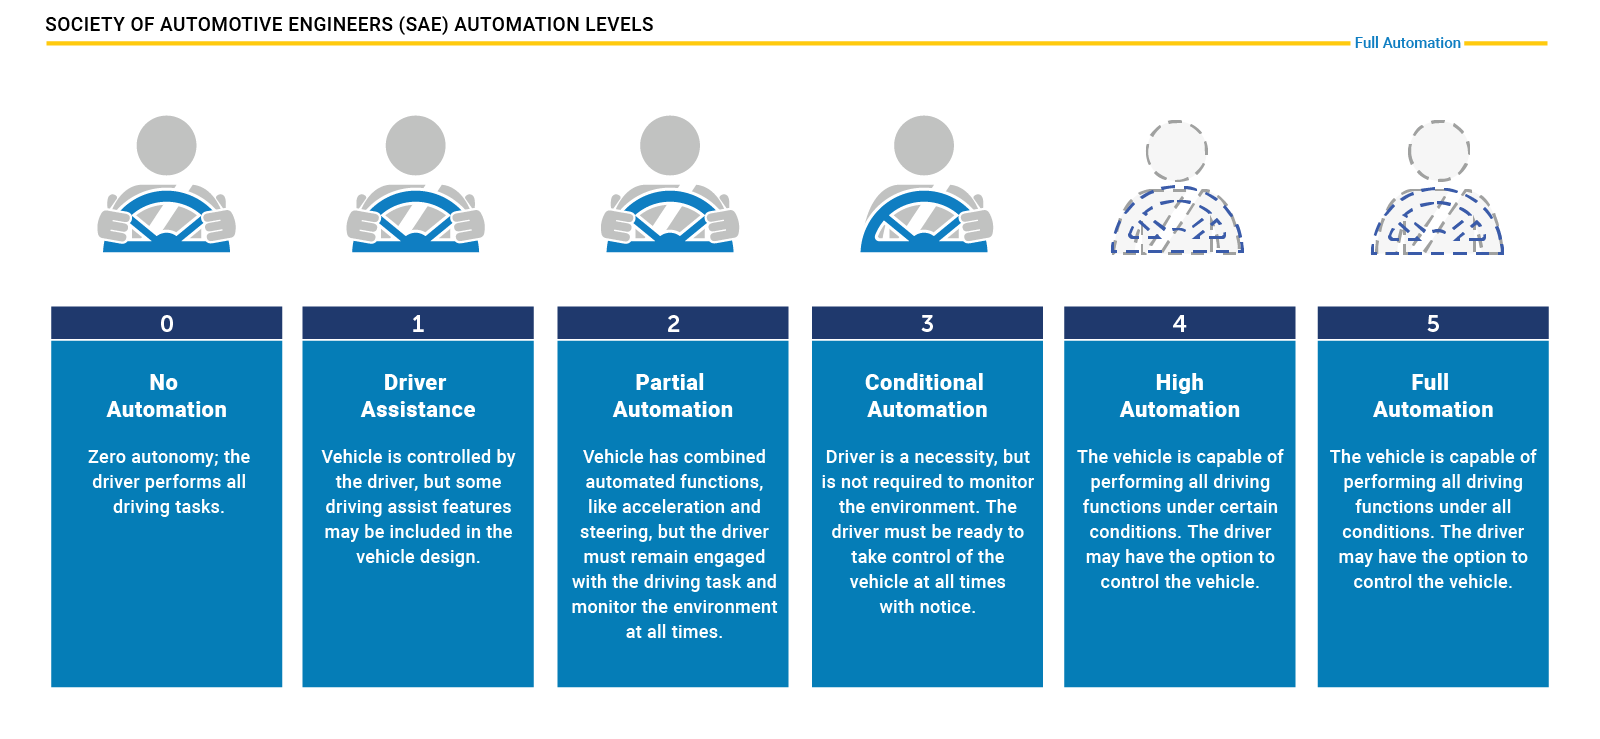
\includegraphics[width=\linewidth]{fotos/autonomia.png}
 %     \caption*{Fonte: https://www.nhtsa.gov/}
 %  	  \label{fig:typesAgent}
 %   \end{figure}

  
\begin{itemize}
    \item Operações de gerenciamento de alunos, professores, turmas. Tal funcionalidade é restrita ao administrador. Lembra que uma turma em 2019 não é exatamente a mesma turma em 2020.
    
    \item Operações de login. Caso o usuário tenho esquecido sua senha ou login, o sistema permitirá a ele o reenvio da senha ou login.
   
    \item O sistema registra todos os eventos realizados pelos usuários contendo informações como usuário, data e hora, nome da funcionalidade, módulo, tipo de operação (inclusão, alteração e exclusão, entre outras). Cada evento realizado poderá ser consultado pelo administrador.
   
    \item O administrador é responsável por montar as turmas podendo adicionar ou excluir um aluno de determinada turma. As turmas indicam a junção de alunos que tenham as mesmas característica em termos de deficiência. Uma turma tem no máximo 15 alunos e pode ter aula com vários professores. Por exemplo, uma turma tem matéria de informática com um professor e de português com outro. Porém, um professor pode ministrar várias matérias. É dado ao administrador pela equipe de desenvolvimento uma chave para o cadastro das contas de ADMIN.
  
    \item O sistema permite o cadastro de uma nova Matéria (Português, Matemática, entre outras) feito pelo professor.  Os dados necessários são: Nome da Matéria; Grau escolar (podendo ser pré-escolar, escolar ou ambos); Objetivos (breve descrição dos objetivos da disciplina) e Assuntos (temas relacionados à matéria que serão desenvolvidos). As matérias que já estiverem vinculadas com aulas não poderão ser excluídas. Exemplo de cadastro de matéria: 
    
    \begin{itemize}
    \item Nome: Português;
    \item Grau escolar: ambos; 
    \item Objetivo: Desenvolver as capacidades de oralidade, leitura, escrita e produção de texto através de didáticas e abordagens diferentes; 
    \item Assuntos: Alfabeto, vogais e consoantes; construção de palavras e divisão de palavras; letras maiúsculas e minúsculas; etc.
    \end{itemize}
    
    \item Os dados necessários para o cadastro de assuntos são: Nome do Assunto; Descrição (breve descrição do assunto). Um assunto pode ser utilizado por várias matérias, por exemplo, o assunto de planetas pode ser tratado na matéria de geografia e português, do mesmo modo que o assunto de redação pode existir na matéria de português e da matemática. Caracterizando diferentes abordagens para um mesmo assunto.
    
    \item Gerar Aula: nesta funcionalidade estão englobadas as operações de cadastro, atualização, remoção e busca de aulas. Cada aula é montada por um professor e pode ser visualizada como também reutilizada por outro professor. A aula é composta por vários jogos sérios que estão relacionadas com várias matérias. Neste caso, deve-se informar a URL do jogo e o sistema abrirá o aplicativo. 
    
    \item Visualizar e executar a aula: esta é uma atividade realizado pelo aluno. Lembre-se que durante a execução da atividade o sistema deve ser capaz de guardar seus erros e acertos para futuramente gerar um relatório estatístico que estará disponível ao professor.
    
    \item Sera concedido aos administradores uma chave de acesso. Com esta chave é possível criar contas com privilégios de administradores.
    
    \item Quando um usuário simples (alunos e professores) esquecem seus dados de acesso, eles enviam uma solicitação para a equipe de administradores, que prontamente disponibiliza uma senha nova ao usuário.
    
\end{itemize}
%%modelo abaixo

\chapter{PROTOTIPAÇÃO DO SISTEMA ATIVA}
    %%CORRECAO1
    \label{chapter:prototipacao do sitema ativa}
        Tela inicial do sistema. Alunos, professores e administradores podem acessa-lo e todos começam aqui. (\fref{fig:1}). O botão de aluno está em destaque propositalmente, para a melhor visualização do aluno com deficiência intelectual.
       
        \begin{figure}[H]
            \centering
            \captionsetup{width=0.9\textwidth}
            \caption{Menu de Acesso}
            
\includegraphics[width=\linewidth]{fotos/1.jpg}
            \caption*{Fonte: Autoria própria}
            \label{fig:1}
        \end{figure}
        
    \subsection{Telas Relacionadas aos Alunos}
       
        
        Tela de acesso do aluno (\fref{fig:2}). É aqui onde os alunos realizam o acesso ao sistema. A tela possui cores fortes e botões grandes, facilitando o acesso dos alunos.
       
        \begin{figure}[H]
            \centering
            \captionsetup{width=0.9\textwidth}
            \caption{Tela de acesso do Aluno}
            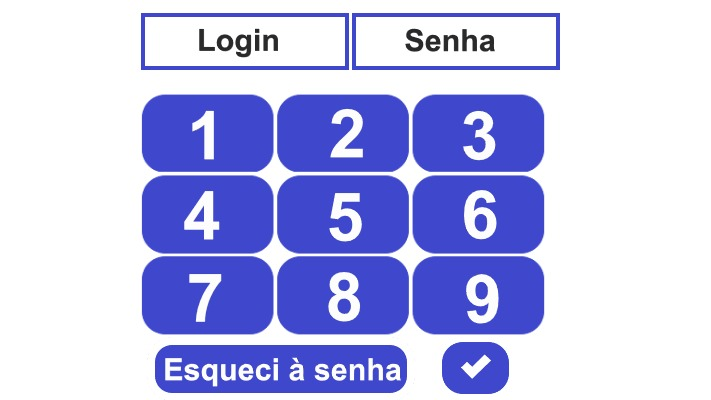
\includegraphics[width=\linewidth]{fotos/2.jpg}
            \caption*{Fonte: Autoria própria}
            \label{fig:2}
        \end{figure}

        Tela de Seleção de Atividades (\fref{fig:3}). Tela onde os alunos realizaram as tarefas. O numero de jogos na tela pode variar dependendo da aula criada pelo Professor. Quando uma atividade é finalizada, sua imagem é oculta da vista, facilitando a progressão do aluno.
       
       
        \begin{figure}[H]
            \centering
            \captionsetup{width=0.9\textwidth}
            \caption{Tela de Seleção de Atividades}
            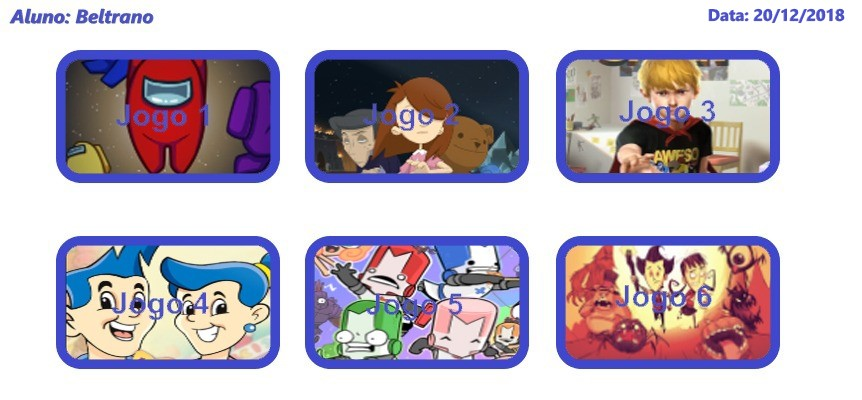
\includegraphics[width=\linewidth]{fotos/3.jpg}
            \caption*{Fonte: Autoria própria}
            \label{fig:3}
        \end{figure}
        Foram utilizadas imagens da internet de jogos, para ilustrar as atividades.
   \subsection{Telas de acesso dos docentes e administradores}
   
        Tela de acesso dos professores e administradores (\fref{fig:4}). Aqui eles realizam o acesso; Solicitam uma nova senha caso tenham esquecido; E, para administradores, realizam o cadastro da conta, com o código de acesso.
       
        \begin{figure}[H]
            \centering
            \captionsetup{width=0.9\textwidth}
            \caption{Tela de acesso dos docentes e administradores}
            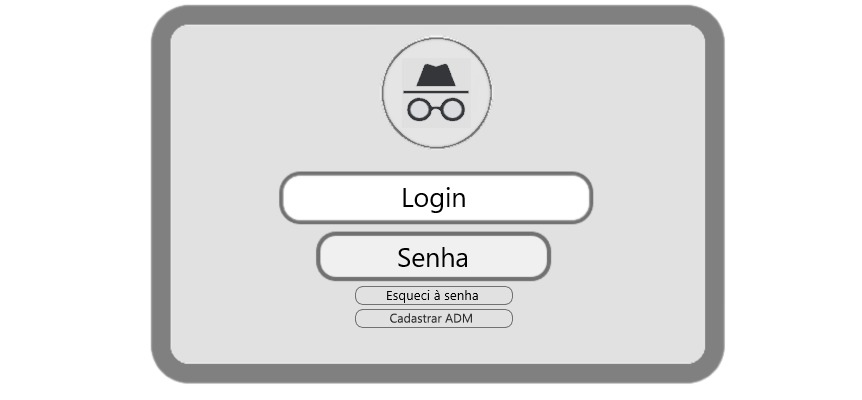
\includegraphics[width=\linewidth]{fotos/4.jpg}
            \caption*{Fonte: Autoria própria}
            \label{fig:4}
        \end{figure}
        
    Tela (\fref{fig:5}) onde os professores solicitam uma nova senha, caso tenham esquecido a antiga, usando o nome ou acesso. A equipe de ADM é notificada.
       
        \begin{figure}[H]
            \centering
            \captionsetup{width=0.9\textwidth}
            \caption{Tela de Solicitação de Nova Senha}
            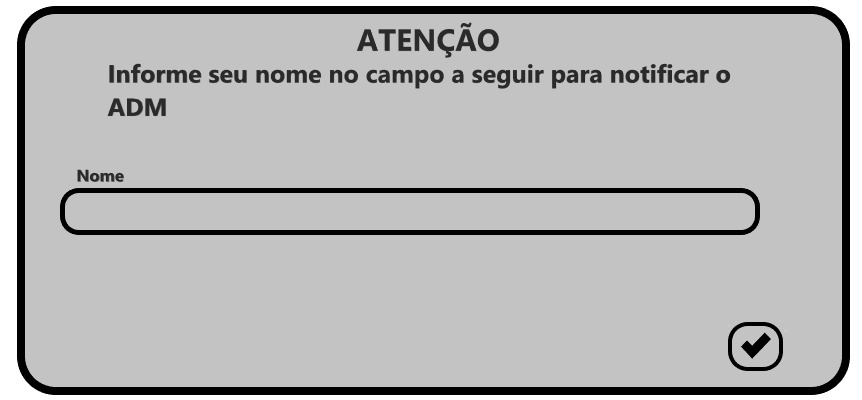
\includegraphics[width=\linewidth]{fotos/5.jpg}
            \caption*{Fonte: Autoria própria}
            \label{fig:5}
        \end{figure}

   \subsection{Telas relacionadas aos Professores}
   
    Tela de menu principal dos professores (\fref{fig:6}). Onde eles podem cadastrar e personalizar aulas, e cadastrar novas matérias.
       
        \begin{figure}[H]
            \centering
            \captionsetup{width=0.9\textwidth}
            \caption{Tela de Menu Principal dos Professores}
            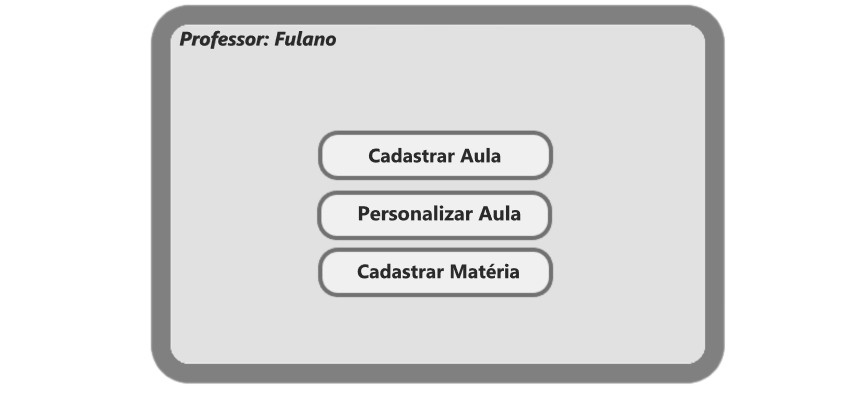
\includegraphics[width=\linewidth]{fotos/6.jpg}
            \caption*{Fonte: Autoria própria}
            \label{fig:6}
        \end{figure}
    
    Tela onde o professor cadastra uma nova matéria (\fref{fig:7}) . O professor, seleciona o grau escolar (é possível selecionar ambos), descreve o objetivo da matéria e seleciona os assuntos que ela ira abordar. Os assuntos podem ser selecionados da lista ou podem ser cadastrados novos assuntos digitando e confirmando com o enter. 
       
        \begin{figure}[H]
            \centering
            \captionsetup{width=0.9\textwidth}
            \caption{Tela de cadastro de Matéria}
            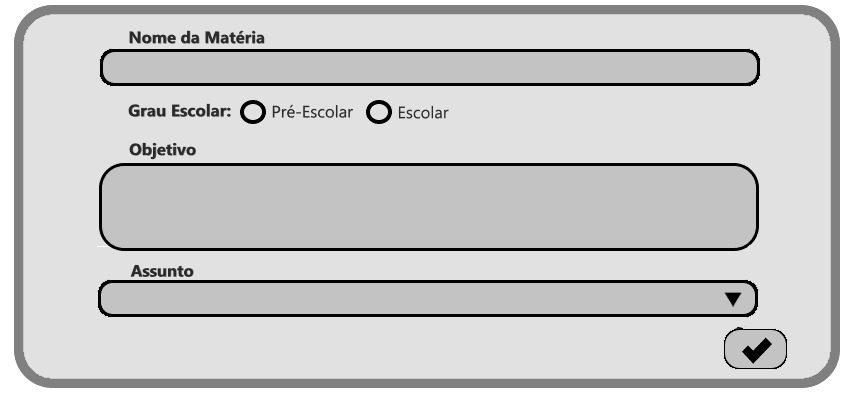
\includegraphics[width=\linewidth]{fotos/7.jpg}
            \caption*{Fonte: Autoria própria}
            \label{fig:7}
        \end{figure}
    
    Tela onde o professor cadastra uma nova aula (\fref{fig:8}). O professor pode inserir jogos , utilizando jogos pré cadastrados anteriormente na lista ou pode cadastrar novos (inserindo o link e pressionando enter); Selecionar uma turma (cadastrada anteriormente pelos ADMS);E selecionar uma Matéria (cadastrada anteriormente pelo professor). Os jogos inseridos na aula aparecem no campo "jogos cadastrados". É dado a aula criada um nome gerado pelo sistema.
      \begin{figure}[H]
            \centering
            \captionsetup{width=0.9\textwidth}
            \caption{Tela de cadastro de Aula}
            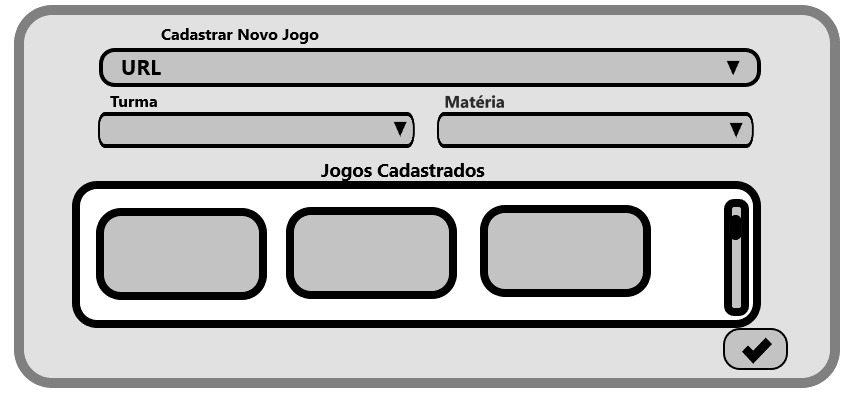
\includegraphics[width=\linewidth]{fotos/8.jpg}
            \caption*{Fonte: Autoria própria}
            \label{fig:8}
        \end{figure}
        
    Tela de personalização das aulas já criadas(\fref{fig:9}). O professor seleciona uma aula cadastrada da lista e pode modifica-la (os outros campos são preenchidos automaticamente). Pode inserir jogos como anteriormente, e agora pode remove-los clicando no simbolo de "X". A turma e a Matéria também podem ser modificadas. Então, o professor, pode atualizar e confirmar ou remover e confirmar.
        \begin{figure}[H]
            \centering
            \captionsetup{width=0.9\textwidth}
            \caption{Tela de Personalização das Aulas Cadastradas}
            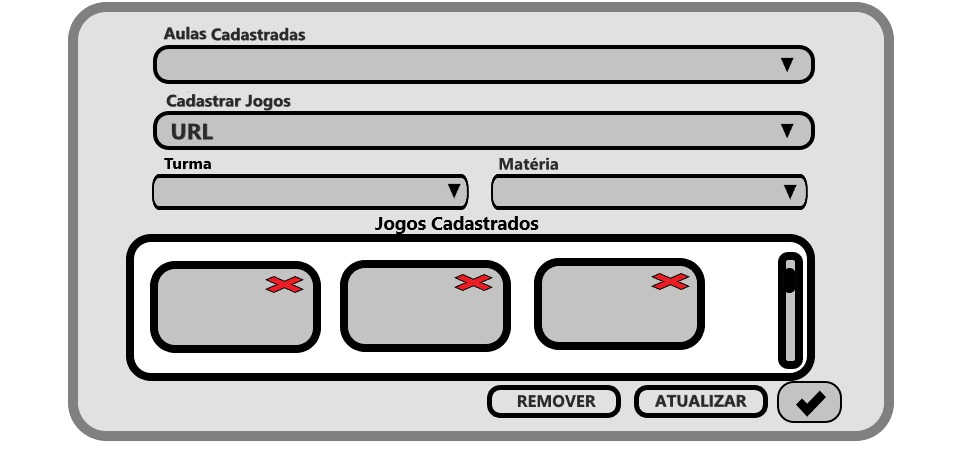
\includegraphics[width=\linewidth]{fotos/9.jpg}
            \caption*{Fonte: Autoria própria}
            \label{fig:9}
        \end{figure}
    
    \subsection{Telas Relacionadas aos Administradores}
    
    Tela de cadastro dos administradores (\fref{fig:10}). Para realizar o cadastro o administrador insere seus dados e o código de acesso fornecido pela equipe de desenvolvimento.
    \begin{figure}[H]
            \centering
            \captionsetup{width=0.9\textwidth}
            \caption{Tela de Cadastro dos Administradores}
            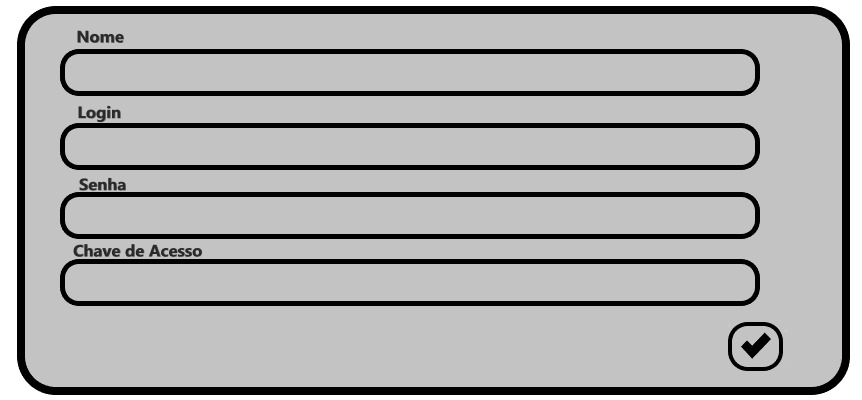
\includegraphics[width=\linewidth]{fotos/10.jpg}
            \caption*{Fonte: Autoria própria}
            \label{fig:10}
        \end{figure}
    Tela de menu principal dos Administradores (\fref{fig:11}). Aqui eles cadastram novos usuários (alunos e professores), personalizam os dados dos usuários (como por exemplo relembrar/modificar a senha), Cadastram e modificam as turmas, e visualizam os logs do sistema.
     \begin{figure}[H]
            \centering
            \captionsetup{width=0.9\textwidth}
            \caption{Tela de Menu Principal dos Administradores}
            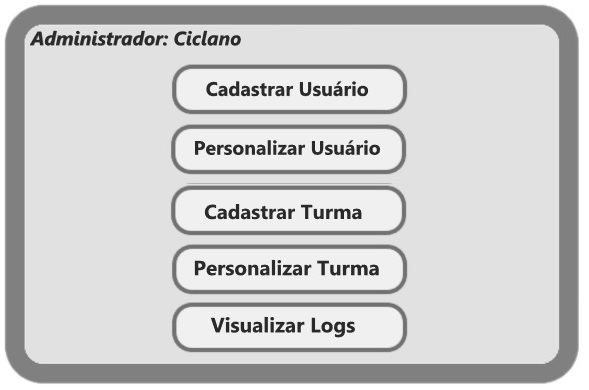
\includegraphics[width=\linewidth]{fotos/11.jpg}
            \caption*{Fonte: Autoria própria}
            \label{fig:11}
        \end{figure}
    
    Tela de logs de eventos (\fref{fig:12}). Aqui os administradores são notificados de tudo o que acontece no sistema. Principalmente quando um professor ou aluno solicita uma nova senha, o administrador é o responsável por modificar a senha e informar o professor.
    \begin{figure}[H]
            \centering
            \captionsetup{width=0.9\textwidth}
            \caption{Tela de Logs do sistema}
            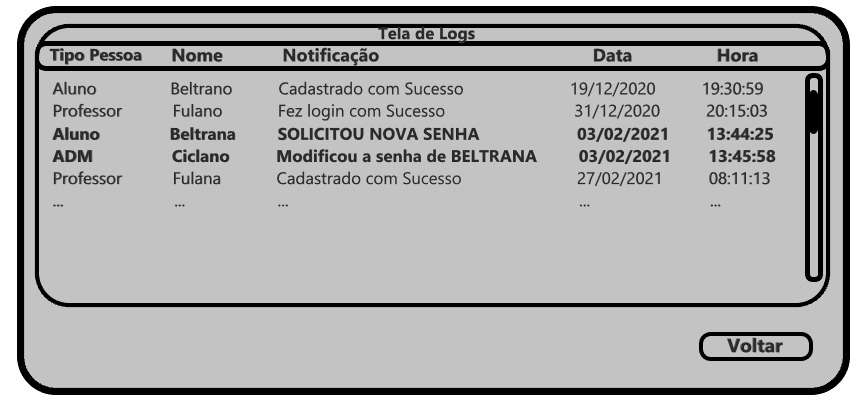
\includegraphics[width=\linewidth]{fotos/12.jpg}
            \caption*{Fonte: Autoria própria}
            \label{fig:12}
        \end{figure}
        
        Tela de cadastro de uma nova pessoa (Professor ou Aluno) (\fref{fig:13}). O cadastro é realizado pelo administrador, que insere os dados da pessoa (fornecidos pelo individuo), seleciona o tipo (professor ou aluno) e confirma.
        \begin{figure}[H]
            \centering
            \captionsetup{width=0.9\textwidth}
            \caption{Tela de Cadastro de usuários}
            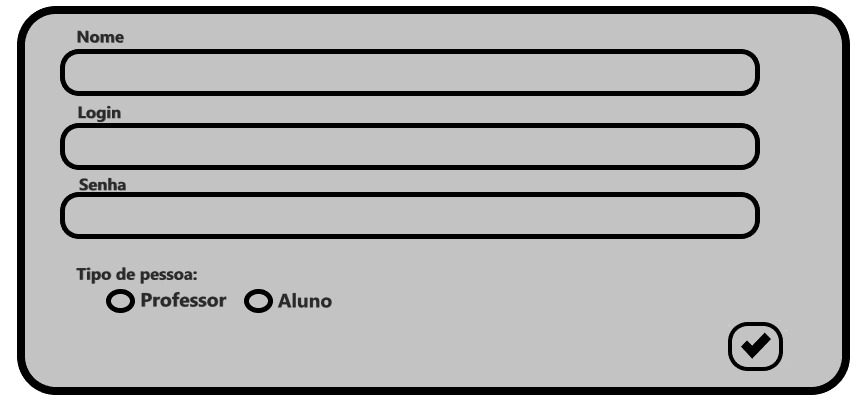
\includegraphics[width=\linewidth]{fotos/13.jpg}
            \caption*{Fonte: Autoria própria}
            \label{fig:13}
        \end{figure}
        
        Tela de personalização de usuários (\fref{fig:13.2}). Aqui o administrador seleciona uma pessoa da lista (os outros campos são preenchidos automaticamente) de nomes e pode modificar todos os dados dela.
        \begin{figure}[H]
            \centering
            \captionsetup{width=0.9\textwidth}
            \caption{Tela de Personalização de usuários}
            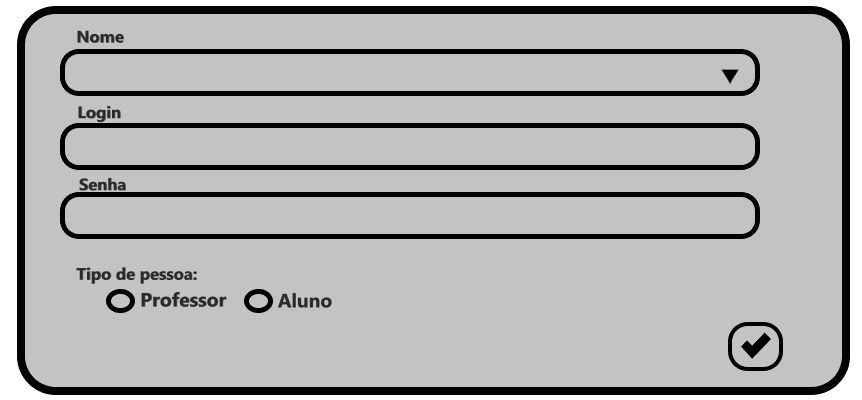
\includegraphics[width=\linewidth]{fotos/13.2.jpg}
            \caption*{Fonte: Autoria própria}
            \label{fig:13.2}
        \end{figure}
        
        Tela de Cadastro de Turmas (\fref{fig:14}). Aqui o administrador seleciona os professores e alunos, e insere na turma (clicando no botão cadastrar ou pressionando enter), insere a data da turma e confirma. Os Alunos e Professores cadastrados na turma são exibidos nas caixas inferiores. É dado, pelo sistema, um nome, gerado automaticamente, a turma cadastrada.
        
        \begin{figure}[H]
            \centering
            \captionsetup{width=0.9\textwidth}
            \caption{Tela de Cadastro de Turmas}
            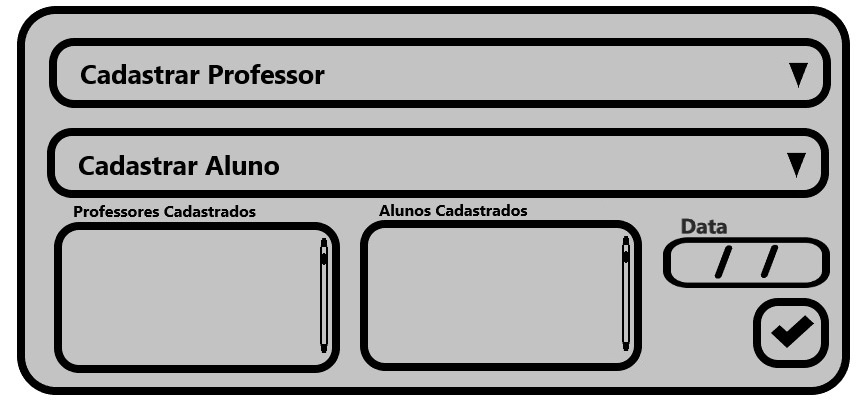
\includegraphics[width=\linewidth]{fotos/14.jpg}
            \caption*{Fonte: Autoria própria}
            \label{fig:14}
        \end{figure}
        
        Tela de Modificação de Turmas (\fref{fig:15}). Aqui o administrado, apos selecionar da lista de turmas cadastradas (os outros campos são preenchidos automaticamente), pode modificar os dados da turma. Para remover alunos ou professores basta clicar no "X" ao lado do nome. Para finalizar a atualização basta clicar em "Atualizar" e confirmar, e para remover a turma basta clicar em "remover" e confirmar.
        \begin{figure}[H]
            \centering
            \captionsetup{width=0.9\textwidth}
            \caption{Tela de Modificação de Turmas}
            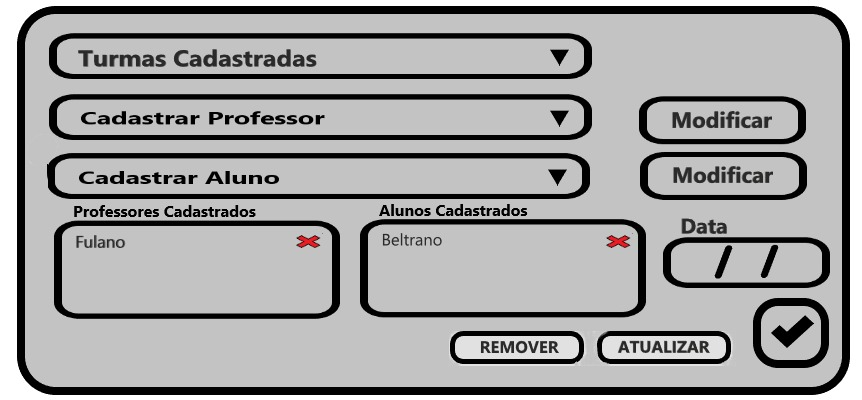
\includegraphics[width=\linewidth]{fotos/15.jpg}
            \caption*{Fonte: Autoria própria}
            \label{fig:15}
        \end{figure}
        
\chapter{DIAGRAMA DE CASO DE USO PARA O SISTEMA ATIVA}
  \label{chapter:diagrama de cado de uso para o sistema ativa}
  Este capítulo exibe o diagrama de caso de uso para o Sistema Ativa.
    \begin{figure}[H]
            \centering
            \captionsetup{width=0.9\textwidth}
            \caption{Diagrama de Caso de Uso para o Sitema Ativa}
            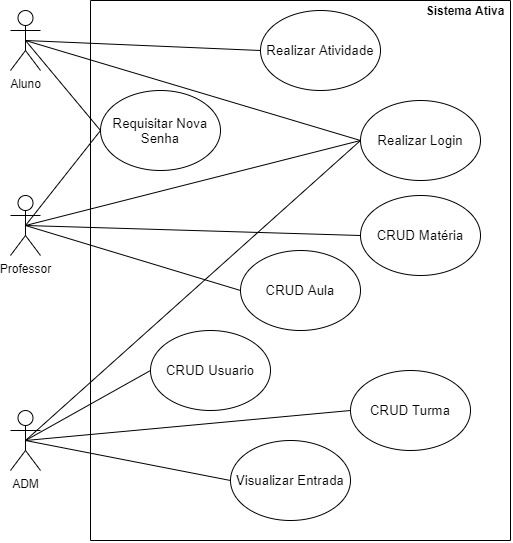
\includegraphics[width=\linewidth]{fotos/Diagrama.jpg}
            \caption*{Fonte: Autoria própria}
            \label{fig:Diagrama de Caso de Uso}
        \end{figure}
 
\bibliography{ref}

\end{document}
